\documentclass[12pt,a4paper]{article}
\usepackage[utf8]{inputenc}
\usepackage[english]{babel}
\usepackage{amsmath}
\usepackage{amsfonts}
\usepackage{amssymb}
\usepackage{graphicx}
\graphicspath{ {./graphics/} }

\usepackage{fullpage}

\usepackage{float}

\usepackage{tikz}
\usetikzlibrary{arrows,automata, positioning,calc,shapes.geometric}
\usepackage{varwidth} % for the diagram of fpga design

\begin{document}

\title{Brick Sorter}
\date{2$^{nd}$ November 2015}
\author{Aitor Miguel Blanco and Lukas Chr. M. W. Schwartz}
\maketitle

\pagebreak

\tableofcontents

\pagebreak

\section{Introduction}

In this project, the problem of solving automatically the sokoban game has been faced.
To do this, the project has been divided in two different parts, being studied separately.
These are finding the shortest solution given a sokoban map and the hardware implementation of a robot able to execute the generated path.

The system loads a map and finds a solution offline with a solver. 
The output of this program is a path that the robot should follow. 
This path is loaded onto the robot, which is prepared to execute it on the sokoban map.

The robot designed is made using different LEGO and LEGO Mindstorms parts and an NXT as controller.
And the solver is programmed using C++.

%The solver is based in the A* algorithm and implemented in C++.


\section{Circuit and Physical Design}

\subsection{Power Supply}
The power supply has been build to deliver three different voltage levels of 5V, 6V and 12V, ensuring a current of 1A, 1.5A and 1A respectively.

This circuit has been printed in a PCB that can be plugged directly into the breadboard to deliver the required voltage and current.
The schematics of such can be seen in figure \ref{fig:powersupply_schematics}.

\begin{figure}[H]
\centering 
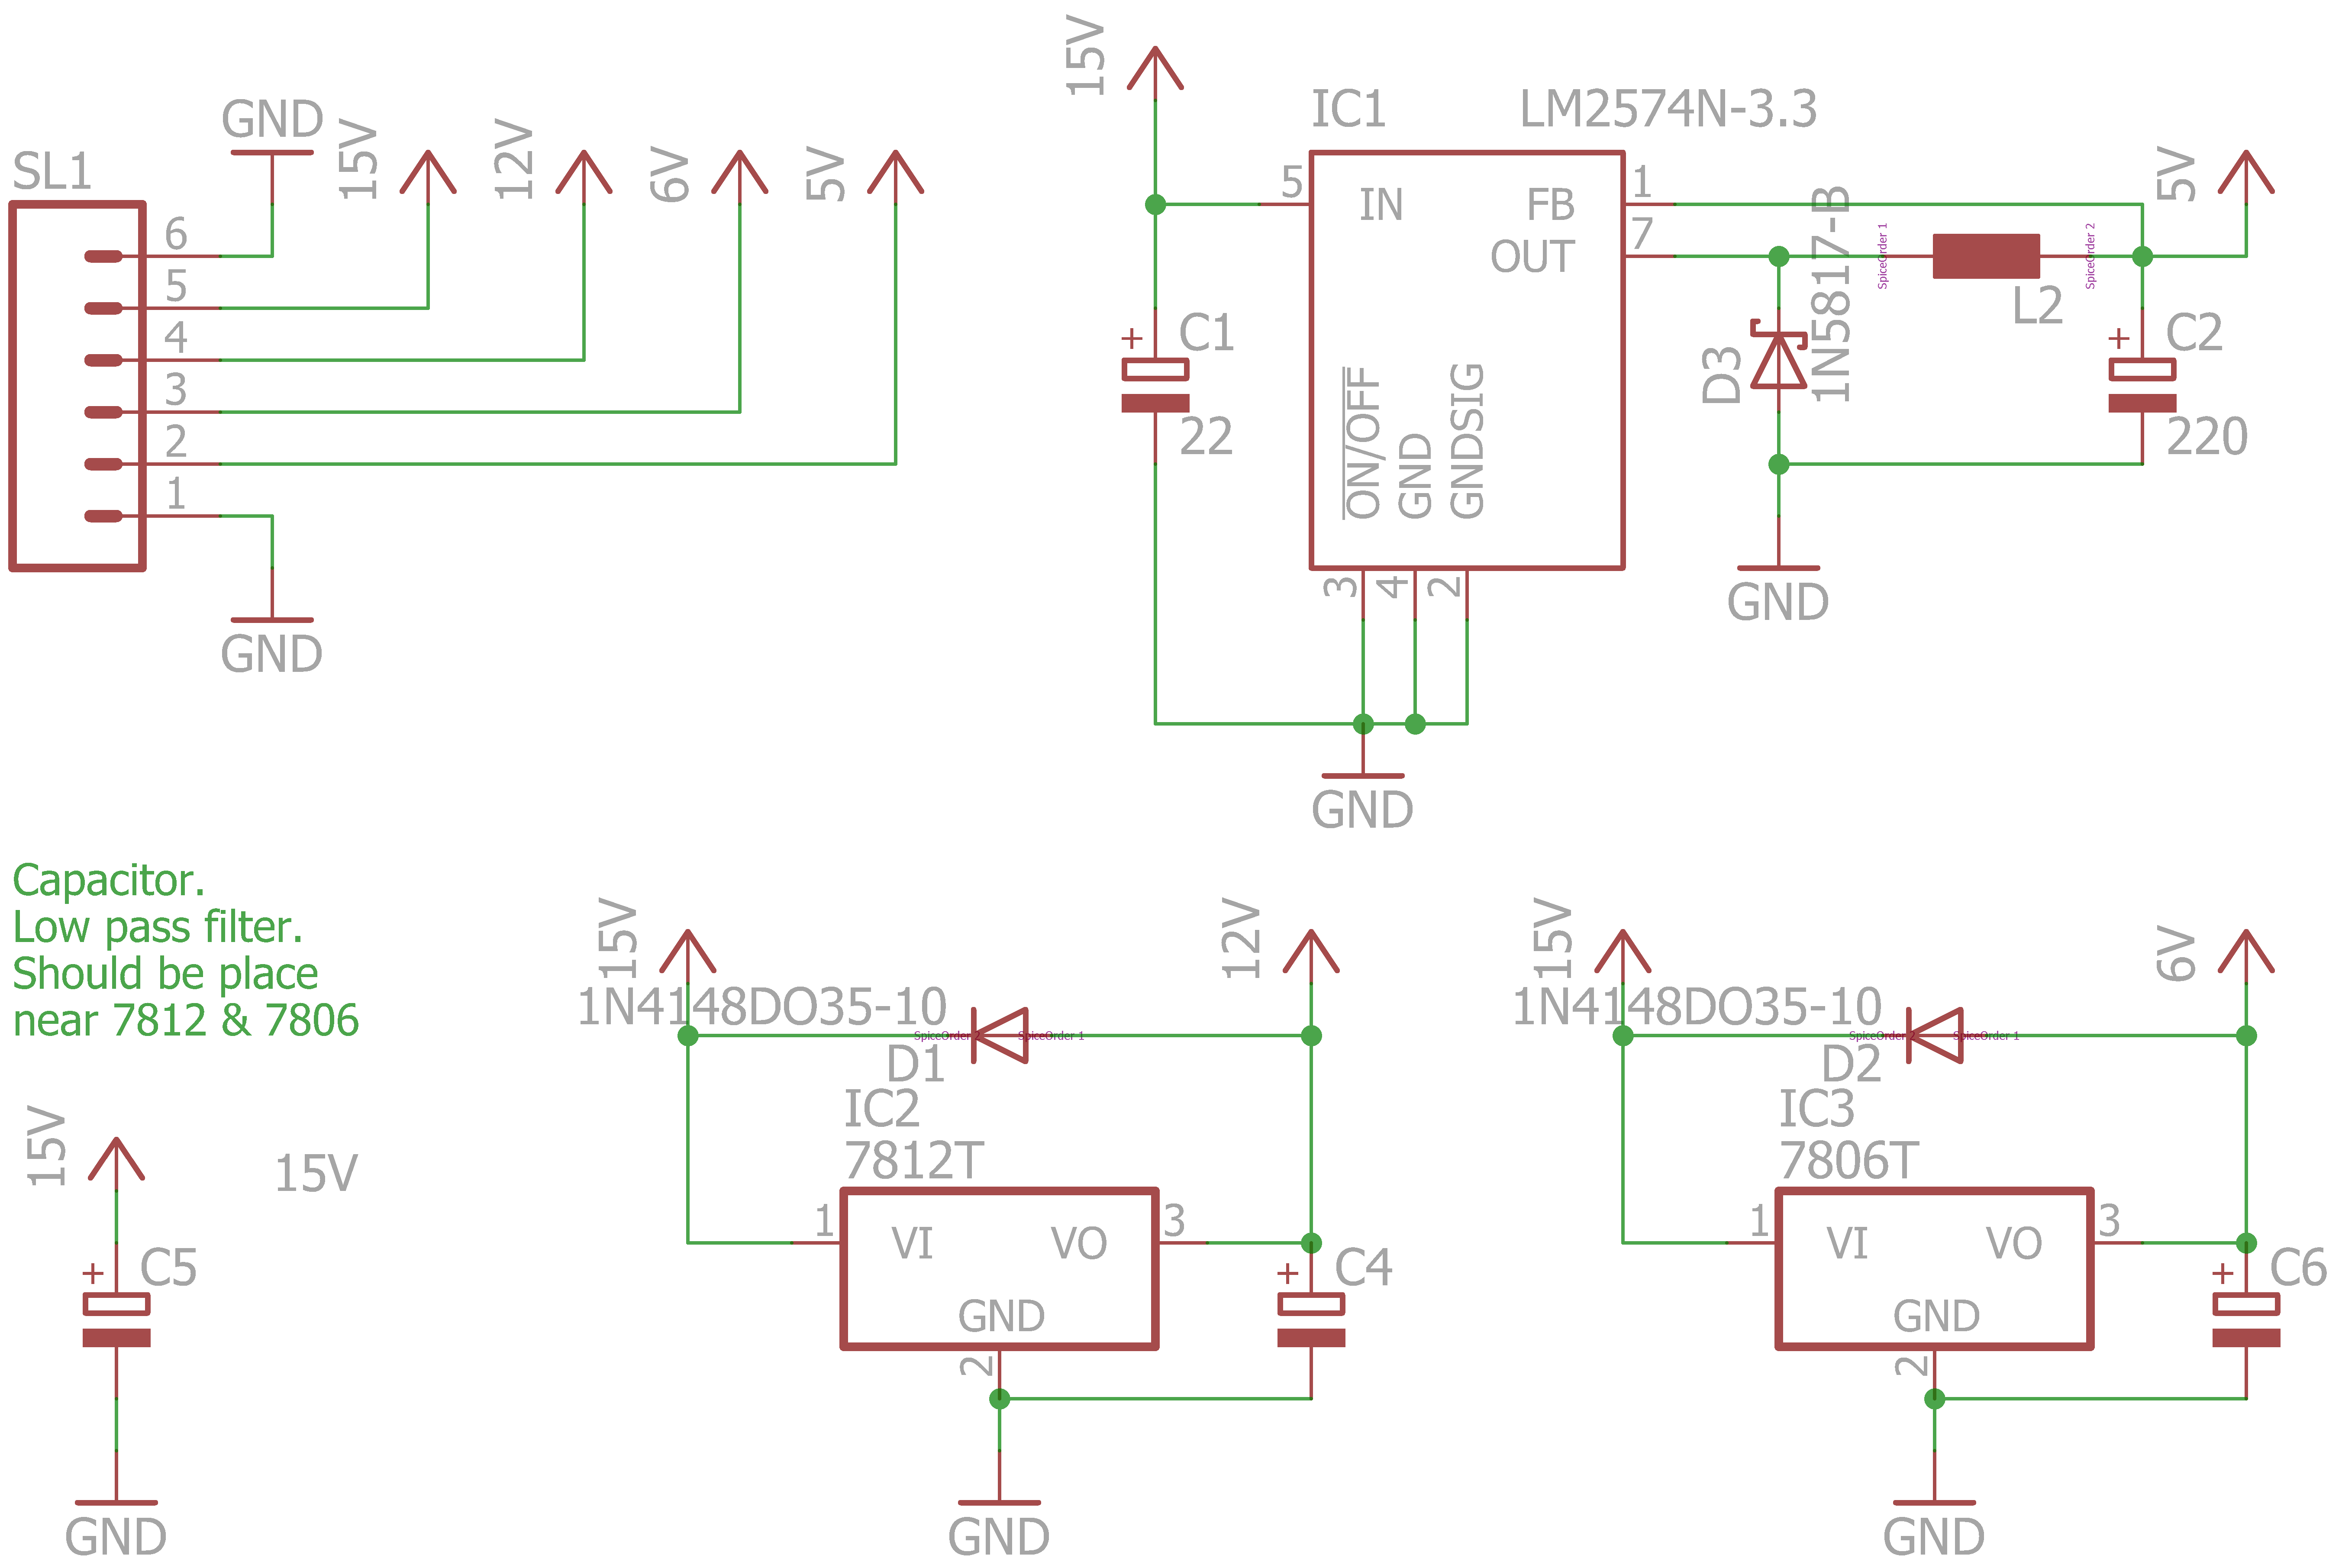
\includegraphics[width = 0.7 \textwidth]{images/powersupply_schematics}
\caption{Schematics of the power supply.}
\label{fig:powersupply_schematics}
\end{figure}


The power supply is connected to a 15V power supply as a input voltage. 
To convert this 15V into 12V, 6V and 5V three different elements are used.
To ensure a 5V/1A supply with a $\pm 1.5\%$ voltage for the FPGA, an LM2574 regulator is used. 
For the 6V/1.5A and 12V/1A, the 7806 and 7812 regulators are used. 
As the efficiency of these regulators is not as good as the one of the LM2574 and they dissipate the excess of power by heating up, a heat-sink for these is required.

The 7806 and 7812 both have a working temperature of maximum $125^{\circ} C$.
In order to hold the temperature of the voltage regulators below this, a heat sink able to dissipate all the heat at the maximum supply rates should be used.

The total energy dissipated by the two regulators can be found by equation \ref{eq:powersupply_energy_dissipation}.

\begin{equation}
P = V_{7806} \cdot I_{7806} + V_{7812} \cdot I_{7812} = (15 - 6) \cdot 1.5 + (15 - 12) \cdot 1 = 16.5W
\label{eq:powersupply_energy_dissipation}
\end{equation}


Estimating the surrounding temperatures to be around $25^{\circ} C$, then the heat sink must keep the temperature below $100^{\circ} C$ rise when $21W$ is dissipated.
This results in a heat sink capable of rising less than $6 ^{\circ}K/W$ is needed to cool the two regulators.
The \textit{Heatsink SK68 100mm 3K/W TO220}\footnote{\href{http://dk.rs-online.com/web/p/koleplader/1898482/?searchTerm=Heatsink+SK68+100mm+3K\%2FW+TO220&relevancy-data=636F3D3226696E3D4931384E44656661756C74266C753D6461266D6D3D6D61746368616C6C7061727469616C26706D3D5E5B5C707B4C7D5C707B4E647D5C707B5A737D2D2C2F255C2E5D2B2426706F3D3926736E3D592673743D4B4559574F52445F4D554C54495F414C5048415F4E554D455249432673633D592677633D4E4F4E45267573743D4865617473696E6B20534B3638203130306D6D20334B2F5720544F32323026}{SK68 100mm 3K/W TO220 Datasheet}} was chosen to do this.
With a $3^{\circ}K/W$ heating coefficient it should be capable of keeping the two regulators at $75^{\circ}C$ during operation with the full load and at a $25^{\circ}C$ ambient temperature.



To test the three power supplies, different loads was added to the outputs of the supplies to check if they meet the specified requirements.
The voltage supplied by the regulators was measured by an oscilloscope and the average recorded for the given load.
The results are seen in figure \ref{fig:voltagesupply}.

\begin{figure}[H]
\centering
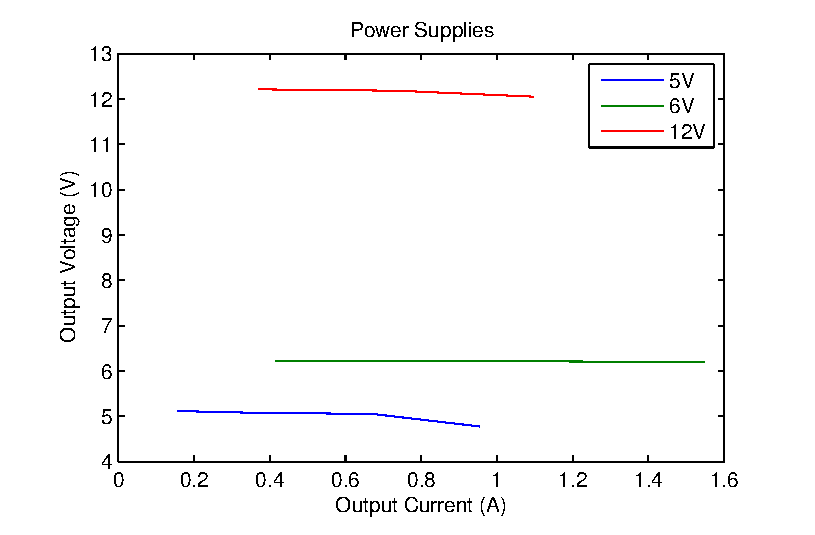
\includegraphics[width = 0.9 \textwidth]{images/powersupply_output}
\caption{Voltage output of the voltage regulators with different loads.}
\label{fig:voltagesupply}
\end{figure}

As seen in figure \ref{fig:voltagesupply} then the power supplies supply a voltage slightly less than desired when exposed to the full load, but as this decreases the voltage reaches the desired voltage.
This might not be desirable, but it is deemed good enough for the project since the power supply rarely, if at all, will be used with full load.


Furthermore the efficiency of the 5V power supply was calculated.
This was done using equation \ref{eq:powersupply_efficiency}.

\begin{equation}
Efficiency = \frac{P_{out}}{P_{in}} = \frac{V_{out}^2 / R_{out}}{V_{in} \cdot I_{in}}
\label{eq:powersupply_efficiency}
\end{equation}

Where, in equation \ref{eq:powersupply_efficiency}, V is the voltage (V), R the load ($\Omega$) and I the current (A) for the circuit where \textit{in} is what was supplied by the 15V supply and \textit{out} the output of the regulator.


\begin{table}[H]
\centering
\begin{tabular}{|c|c|c|c|c|}
\hline
Load ($\Omega$) & Min Efficiency & Avg. Efficiency & Max Efficiency \\ \hline
5 & 0.7806 & 0.7996 & 0.8367 \\ \hline
7.5 & 0.7570 & 0.8095 & 0.8096 \\ \hline
15 & 0.7556 & 0.7640 & 0.8587 \\ \hline
33 & 0.644 & 0.6607 & 0.7318 \\ \hline
\end{tabular}
\caption{Efficiency of the 5V supply.}
\label{tab:voltageefficiency}
\end{table}

The efficiency was calculated considering that the input supply is stable and using the maximum, minimum and average output voltages measured with the oscilloscope.
It can be seen from table \ref{eq:powersupply_efficiency} that the efficiency of the regulator is capable of supplying the voltages at the project requirement of 80\%, for small loads.
As the load increases above $7.5\Omega$ the efficiency decreases considerably.
This is however expectable since the regulator used specifies that the efficiency is highest when driving a load with 0.5A at 5V and then only is specified to achieve the 80\%.



\subsection{LED controller}



\begin{figure}[H]
\centering 
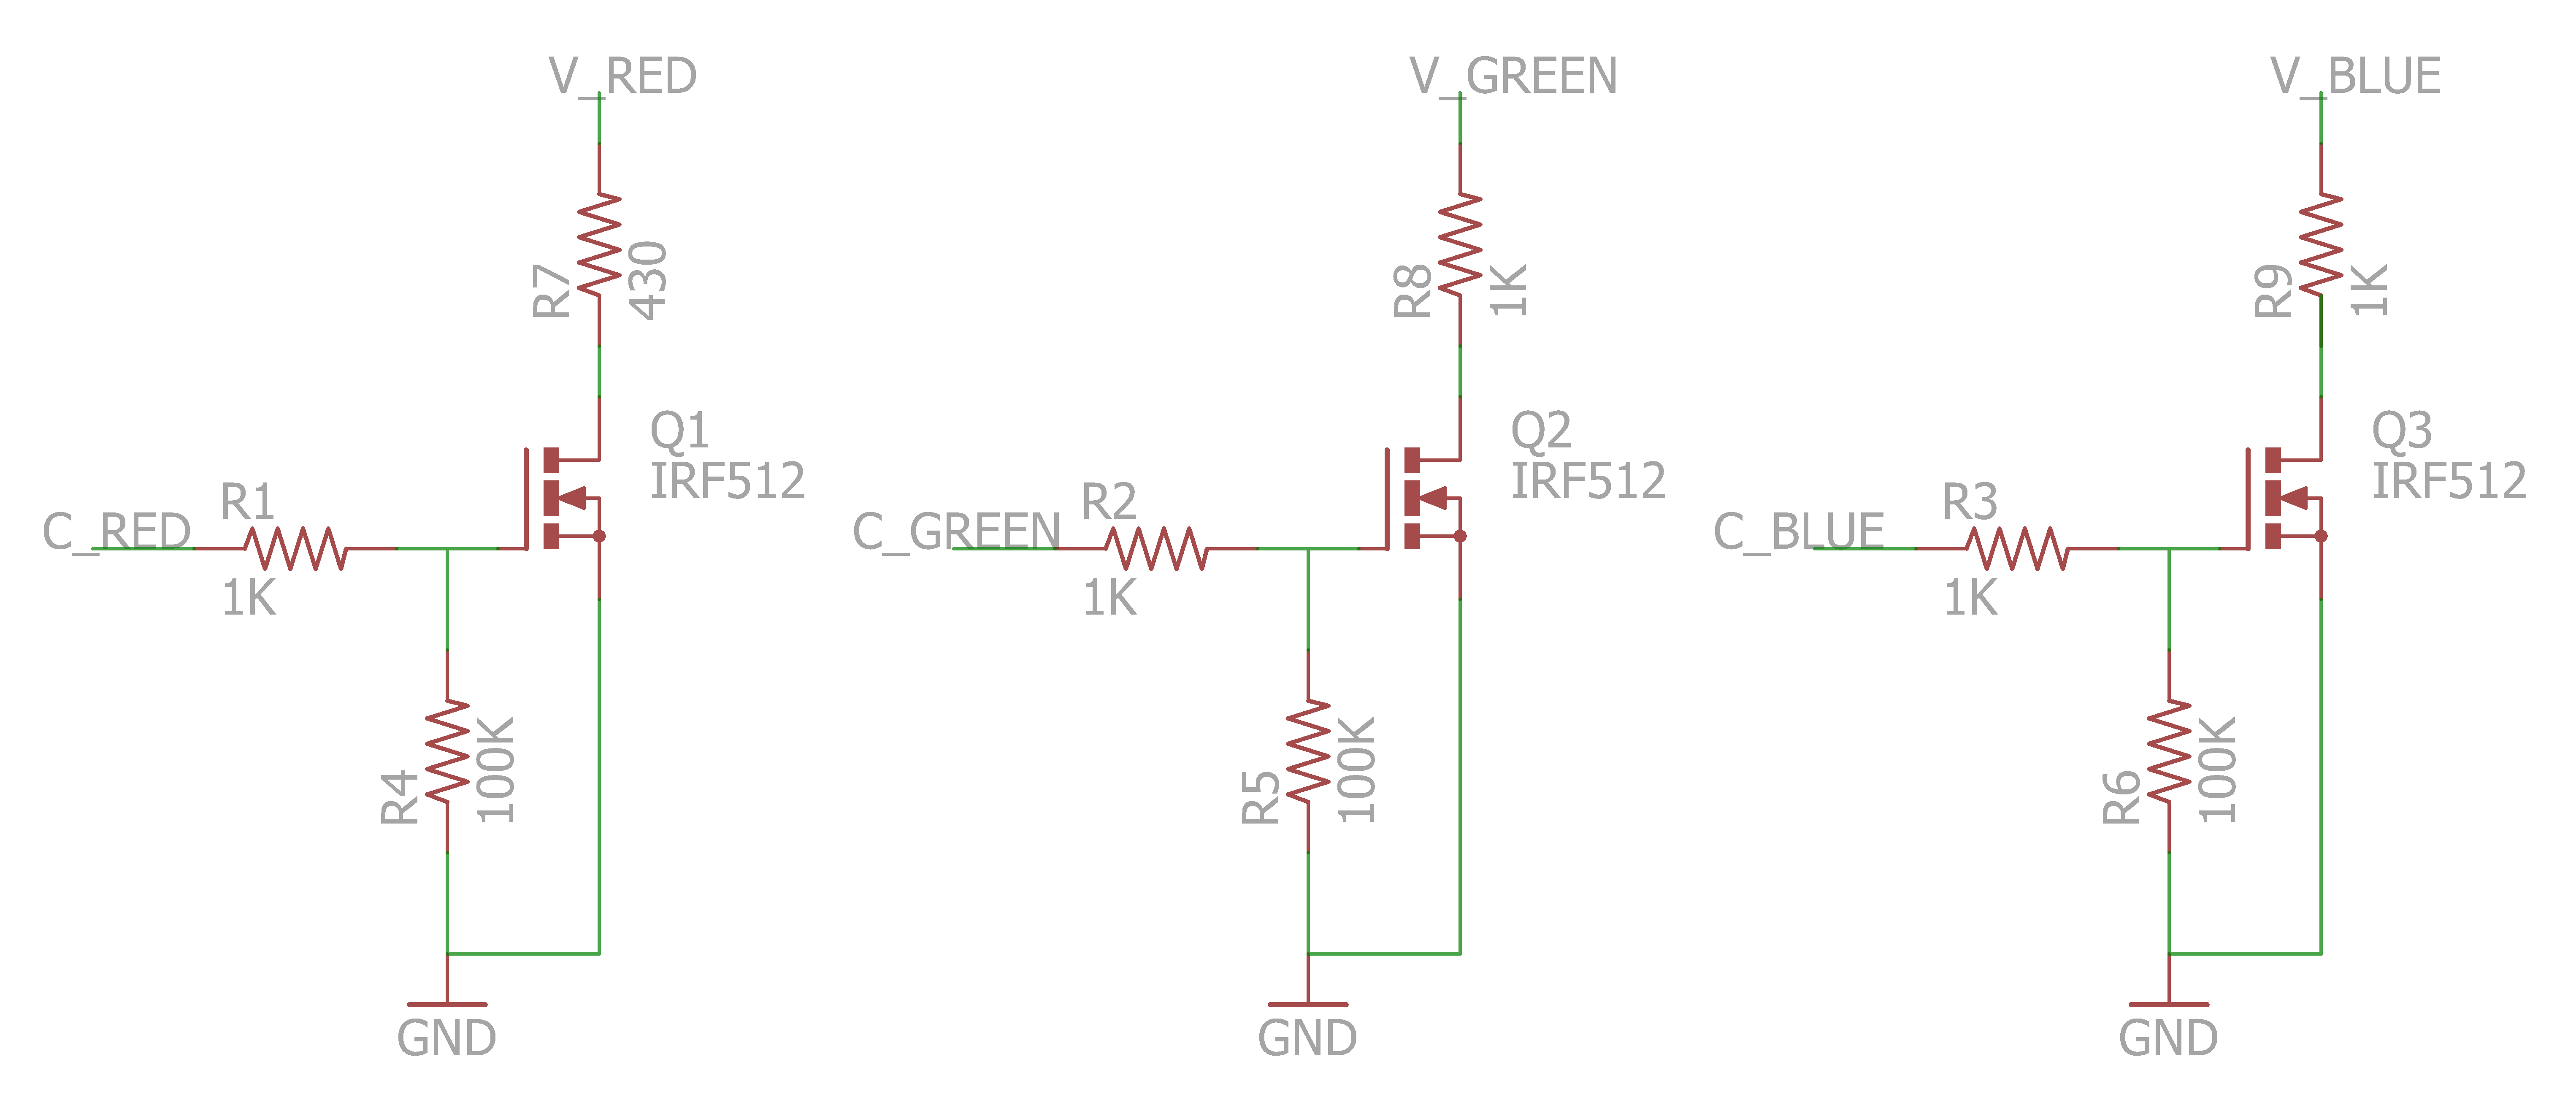
\includegraphics[width = 0.4 \textwidth]{images/leddriver_schematics}
\caption{...}
\label{fig:...}
\end{figure}


\subsection{Light sensor}


\begin{figure}[H]
\centering 
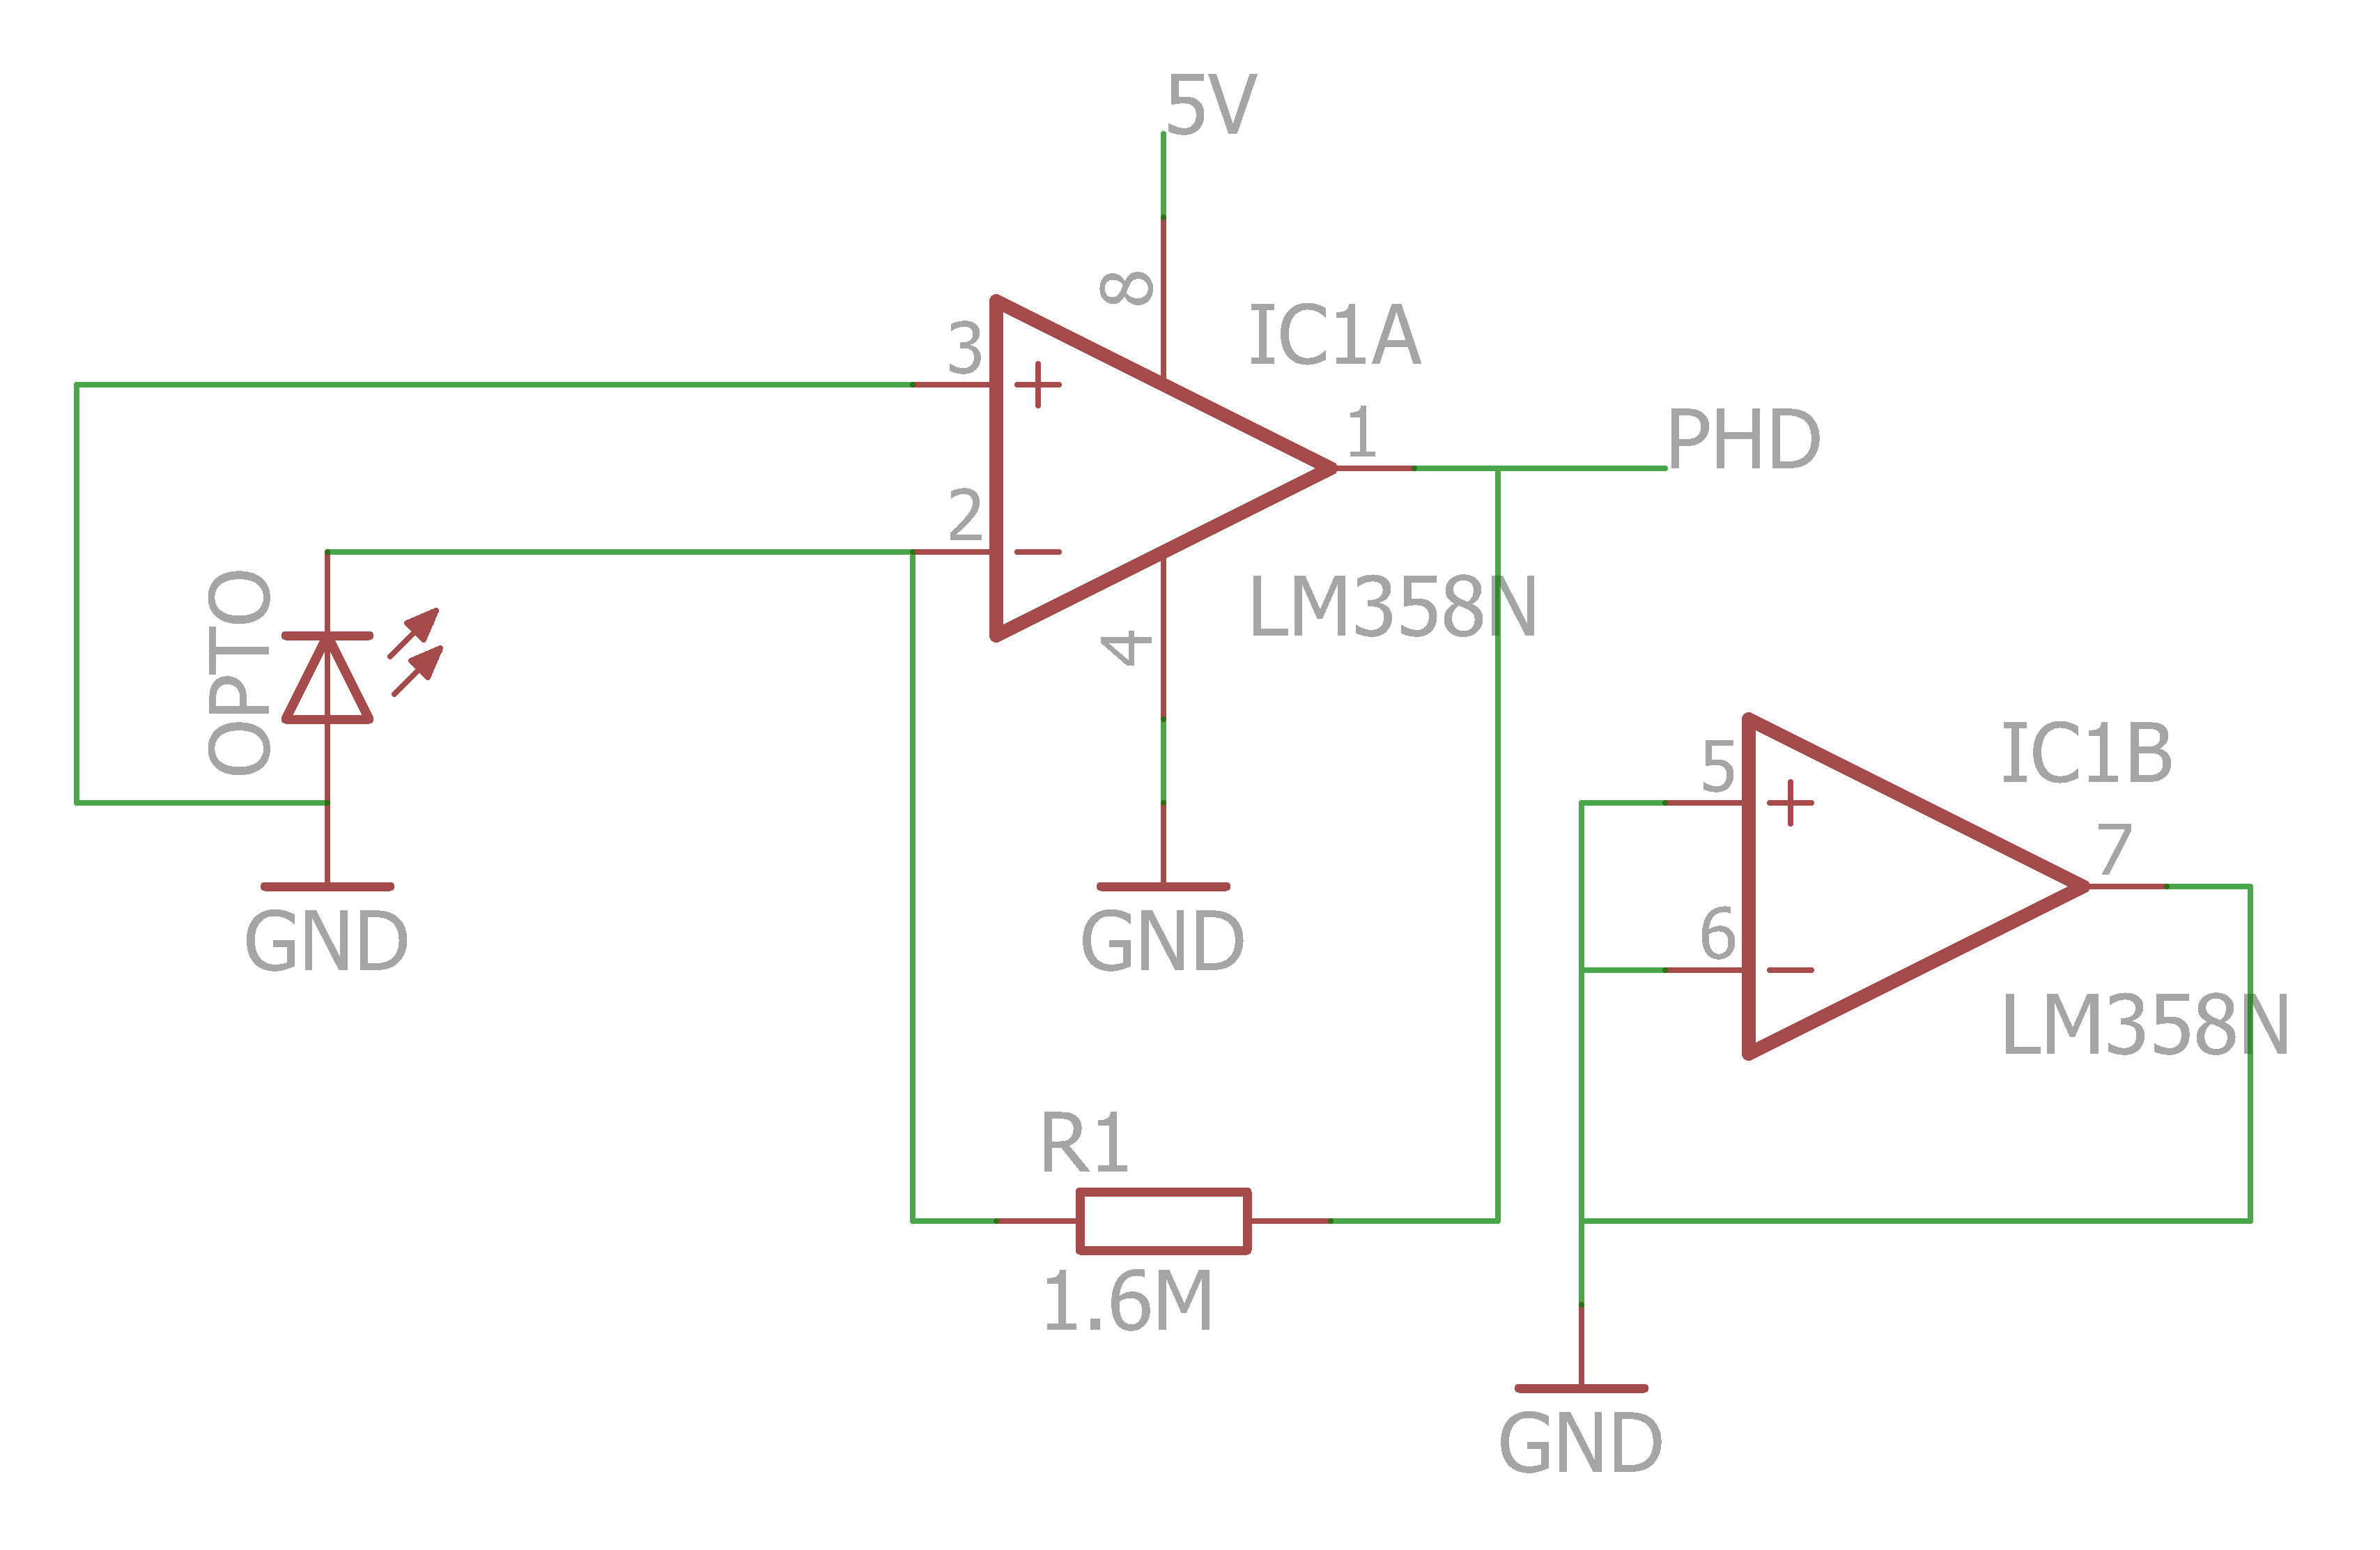
\includegraphics[width = 0.4 \textwidth]{images/optoamplifier_schematics}
\caption{...}
\label{fig:...}
\end{figure}


\begin{figure}[H]
\centering 
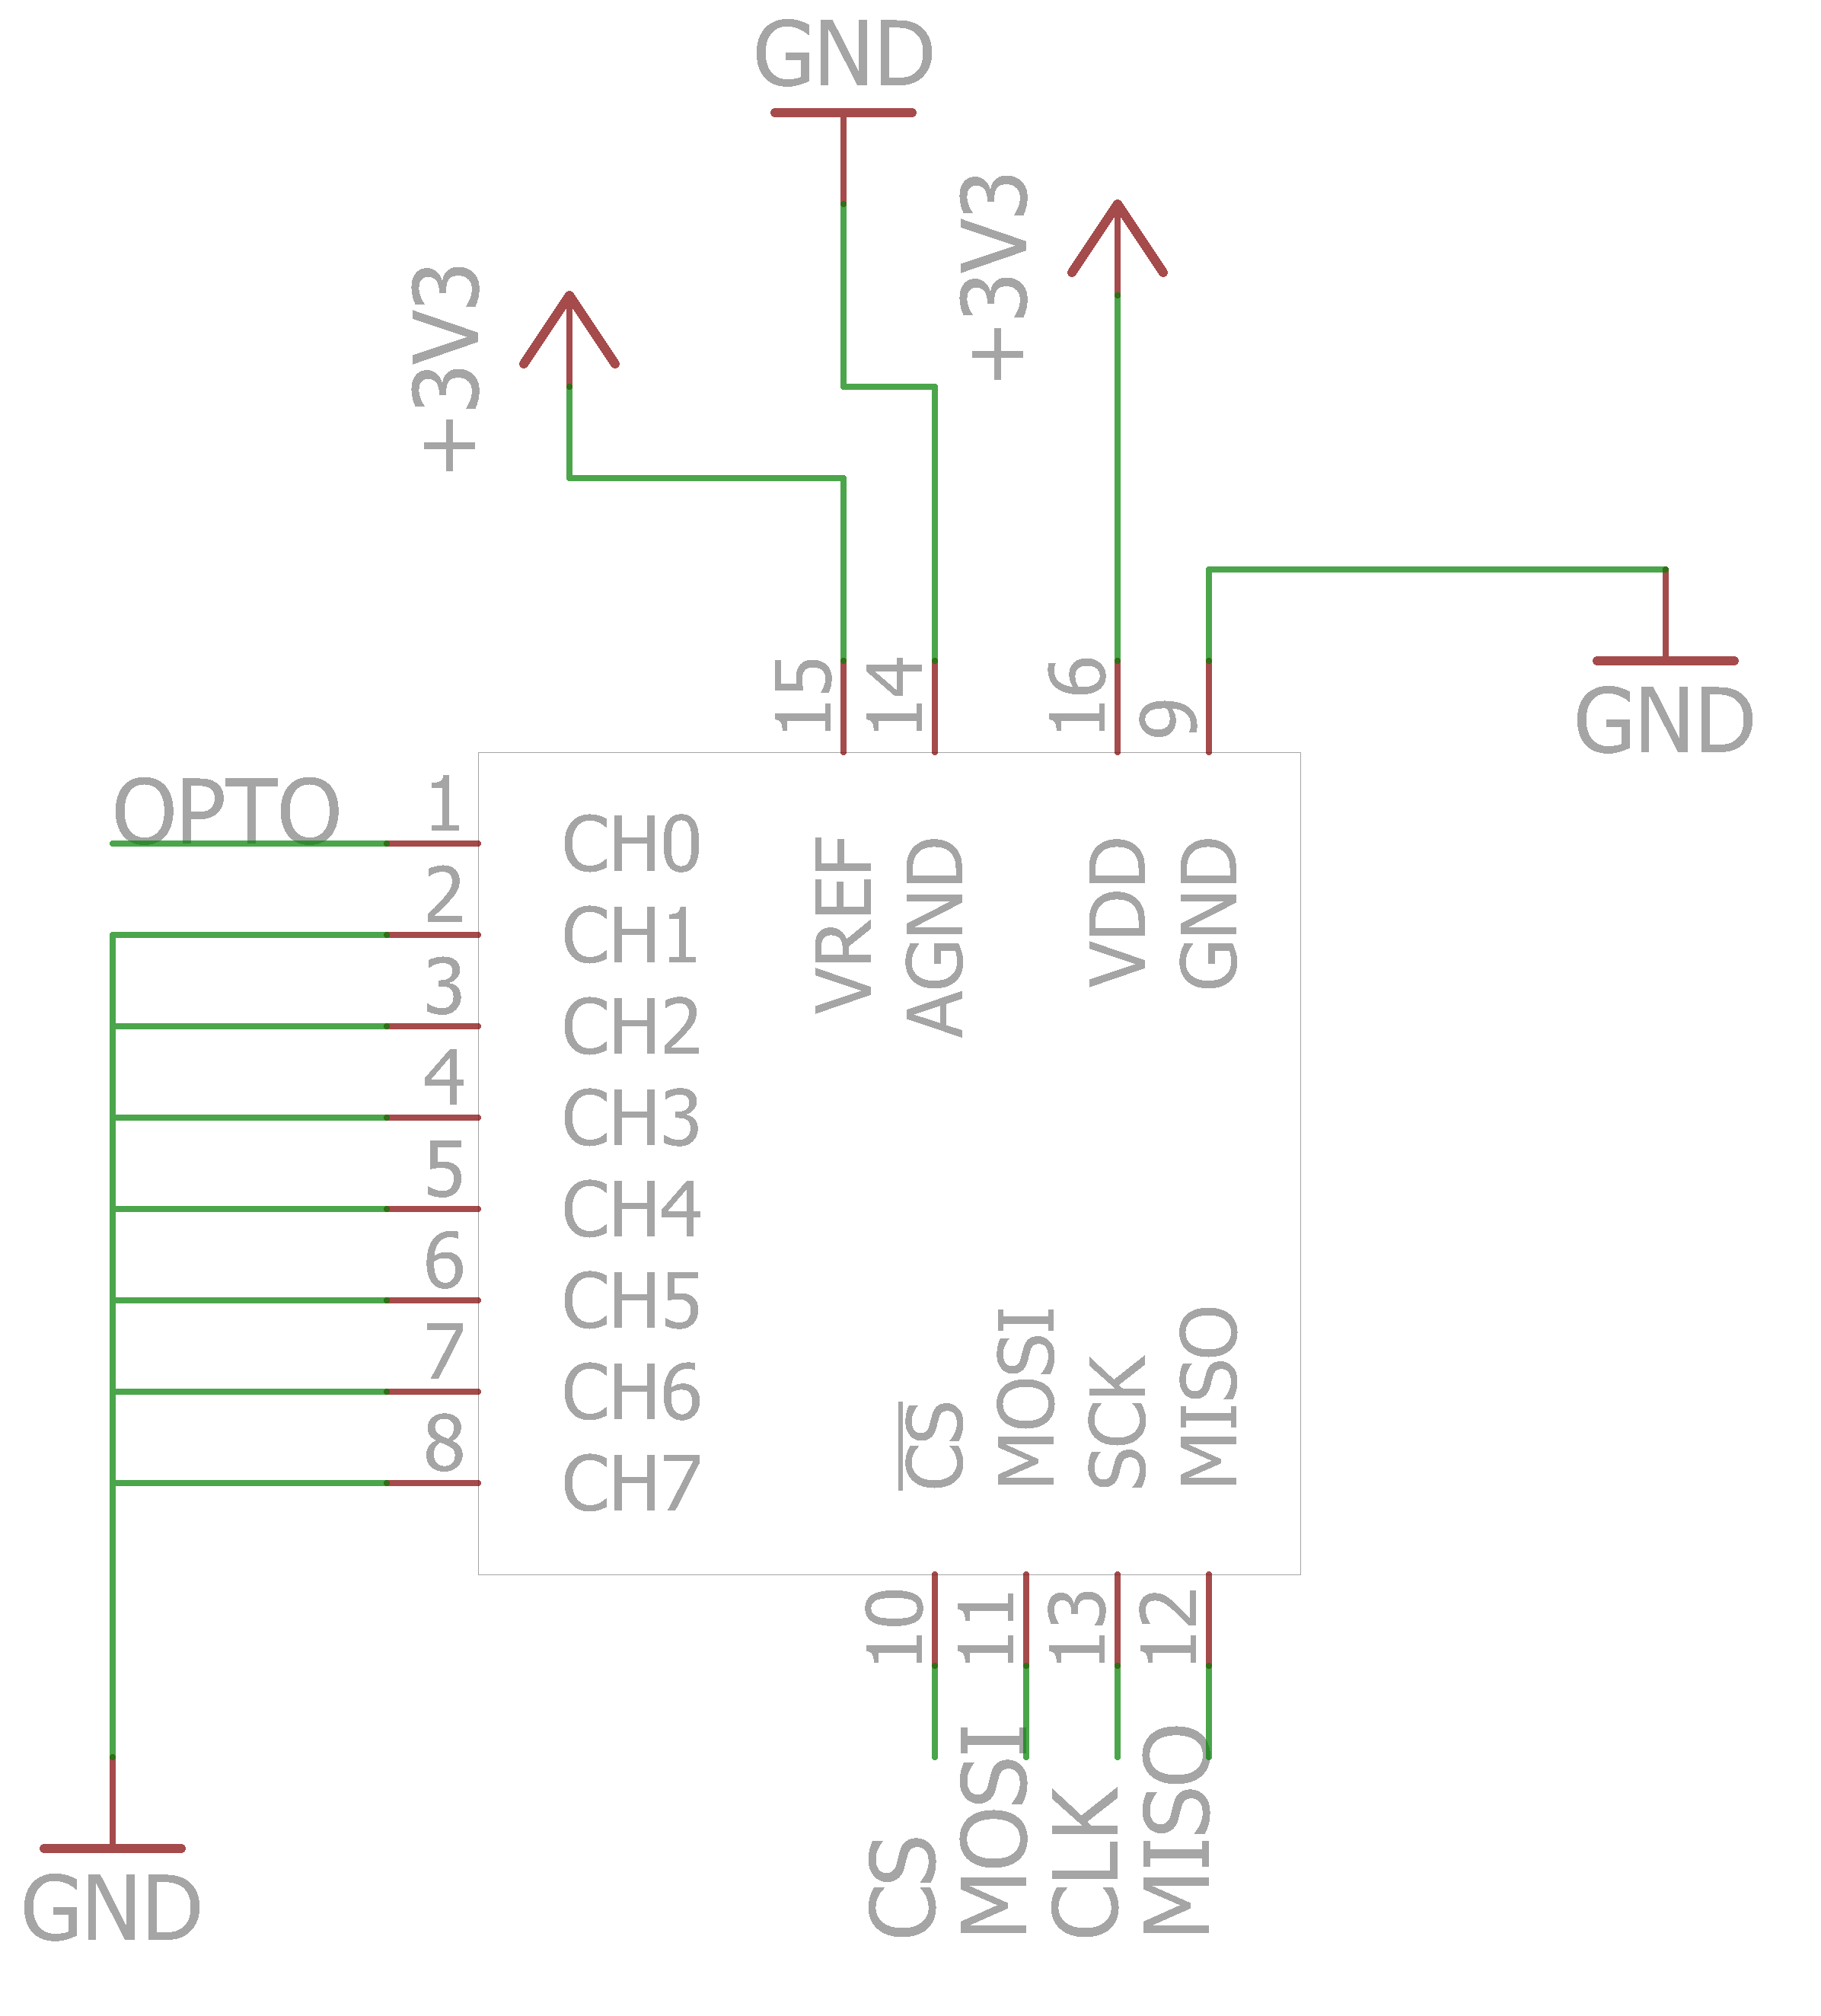
\includegraphics[width = 0.4 \textwidth]{images/ADC_schematics}
\caption{...}
\label{fig:...}
\end{figure}
\subsection{Servo motor}


\section{Software}

In order to control and stabilize the segway a the communication with the accelerometer/gyroscope must be established.
This must data received must then be processed in order to control the motors according to the segways position.



\begin{figure}[H]
\centering

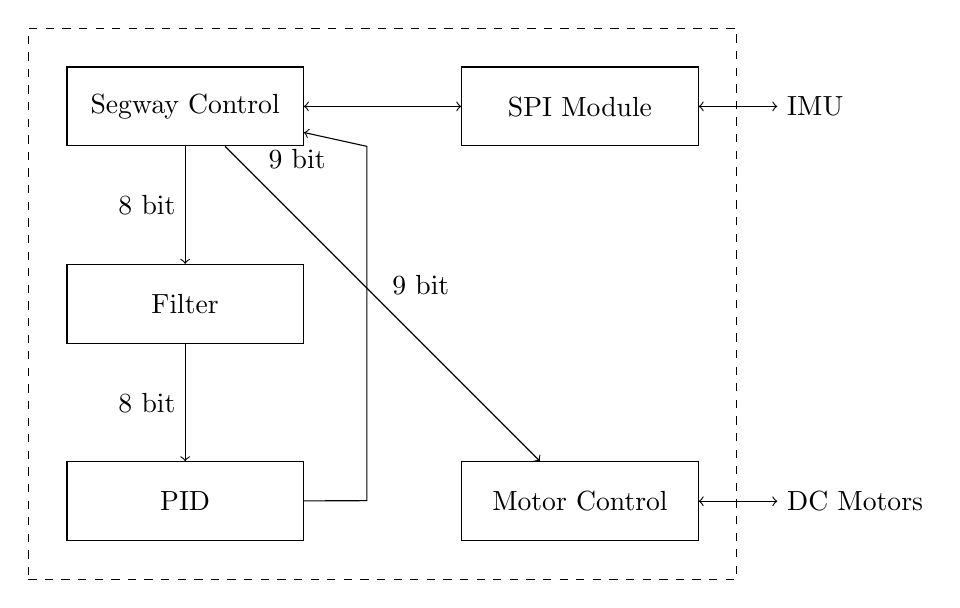
\begin{tikzpicture}[node distance=1cm]
% FPGA border
\node[rectangle,draw,minimum width=9cm, minimum height=7cm, dashed, name=FPGA]  {};

% used to align the insides of FPGA
\node[rectangle,minimum width=5cm, minimum height=5cm, name=FPGAaligne] {};

% components of FPGA
\node[rectangle,draw,minimum width=3cm, minimum height=1cm, name=pid] at (FPGAaligne.-135) {PID};
\node[rectangle,draw,minimum width=3cm, minimum height=1cm, name=communiction] at (FPGAaligne.45) {SPI Module};
\node[rectangle,draw,minimum width=3cm, minimum height=1cm, name=mc] at (FPGAaligne.-45) {Motor Control};
\node[rectangle,draw,minimum width=3cm, minimum height=1cm, name=filter] at (FPGAaligne.180) {Filter};
\node[rectangle,draw,minimum width=3cm, minimum height=1cm, name=segway] at (FPGAaligne.135) {Segway Control};

% nodes outside FPGA
%\node [left=of utos,name=pc] {PC};
\node [right=of communiction,name=spi] {IMU};
%\node [left=of color,name=rgb] {RGB(2:0)};
\node [right=of mc,name=motor] {DC Motors};

% arrows inside FPGA
\draw[<->] (segway) -- node[] {} (communiction) ;
\draw[->] (segway) -- node[left] {8 bit} (filter) ;
\draw[->] (filter) --  node[left] {8 bit} (pid) ;
\draw[->] (segway) -- node[above right] {9 bit} (mc) ;
\draw[->] (pid) --(-0.2,-2.5)--(-0.2,2)-- node[below left] {9 bit} (segway) ;
 
% arrows connected to the outside of FPGA
\draw[<->] (spi) -- node[] {} (communiction) ;
\draw[<->] (mc) -- node[] {} (motor) ;
%\draw[->] (adc) to[out=180, in=0] node[] {} (ad) ;
%\draw[->] (color) to[out=180, in=0] node[] {} (rgb) ;
%\draw[->] (mc) to[out=0, in=180] node[] {} (servo) ;
\end{tikzpicture}

\caption{Block design of the FPGA.}
\label{fig:fpga_sof_design}
\end{figure}


The designed system is comprised by the modules seen in figure \ref{fig:fpga_sof_design}.
Here the \textit{Segway Control} block is the main part of the system, used to combine the different components into one.
The \textit{SPI Module} takes care of the communication with the accelerometer and gyroscope by sending data to such when asked for by the \textit{Segway Control} module.

Data from such is then send to the \textit{Filter} to predict an angle.
From here the angle is passed to the \textit{PID} in order to generate a duty cycle which is then passed back to the main module, the \textit{Segway Control}.
The \textit{Segway Control} hence also takes care to set the right ports on the H-bridges, through the \textit{Motor Control} unit, depending on the speed and direction bit generated by the \textit{PID}.
The five components are explained further throughout this section.


\subsection{Top Module}
The top module is the part of the system which combines all the functionality the FPGA should have.
Its core functionality is implemented as the state machine in figure \ref{fig:topmodule_fsm}.
This state machine is sorting the bricks using the signals generated from the sub components.


\begin{figure}[H]
\centering
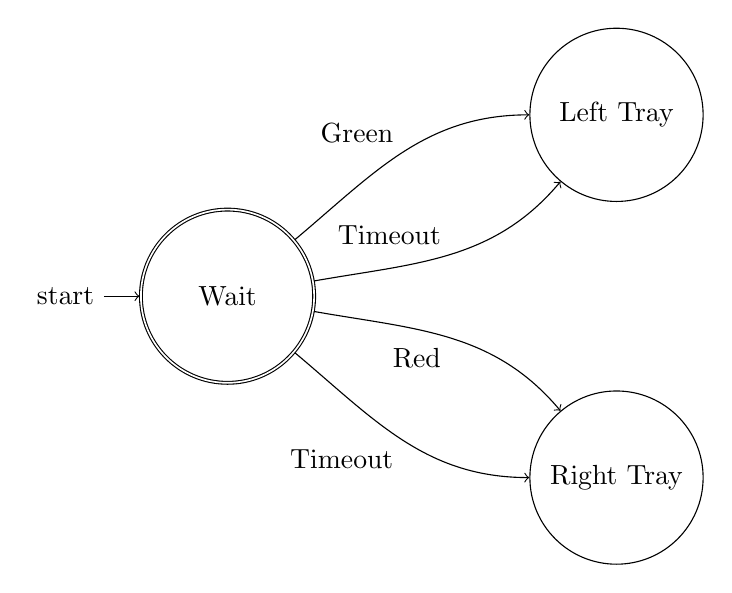
\begin{tikzpicture}[node distance=3cm]
\node[circle, minimum width=6cm, name=c] {};

\node[initial,accepting,state,name=start,minimum width=2.2cm] at (c.180)   {Wait}; 

\node[state,name=left,minimum width=2.2cm] at (c.50)   {Left Tray}; 
\node[state,name=right,minimum width=2.2cm] at (c.-50)   {Right Tray}; 


%\node[name=rst] at (-2.5,3) {rst};

\draw[->] (start) to[out=40, in=180] node[midway,above left] {Green} (left) ;
\draw[->] (start) to[out=10, in=230] node[midway,above left] {Timeout} (left) ;

\draw[->] (start) to[out=-10, in=-230] node[midway,below left] {Red} (right) ;
\draw[->] (start) to[out=-40, in=180] node[midway,below left] {Timeout} (right) ;  
\end{tikzpicture}

\caption{Top module Finite State Machine.}
\label{fig:topmodule_fsm}
\end{figure}


The state machine in figure \ref{fig:topmodule_fsm} waits in the idle mode whenever no brick is or has passed.
When a brick is detected, and the state machine is in the \textit{Wait} state, then it moves to the \textit{Right-} or \textit{Left Tray} state depending on the color of the brick.
When the state is changed, a timer is started and this generated a timeout signal once the time has elapsed.
This timeout results in the state machine returning to its initial \textit{Wait} state when the brick has passed the sorter.
While the state machine is in \textit{Left-} or \textit{Right Tray}, it sends a signal to the \textit{Motor Control} component to move to the left or right side in order to sort the bricks.
Otherwise, the motors are told to return to its initial position, which is when the motor is pointing the sorter towards the falling bricks.
The timeout period before switching back to the \textit{Wait} state was set such that the bricks would have enough time to pass through the sorting mechanism on the slide before the sorter would return to its initial state.




\subsection{AD-Converter Communication}
The ADC communicates using SPI.
This is hence implemented in the module.
Since the ADC only allows up to 3.6MHz communication frequency, then the clock is scaled down to 3.57MHz.
The FPGA is then requesting the data from the ADC continuously and whenever a whole message is received, it is send out into the FPGA and a signal is pulsed to notify the color detector of the new message.
\subsection{Servo motor}
\subsection{PC Communication}









\end{document}